\section{Examples}
% Organize this section according to major topics
% give each topic a section heading in boldface.
% try to cover the major common points :
%
% problem design
% methods of measurement
% supporting models
% supporting data
% simulations run
% results

% Just write the section headings for each part and indicate what goes in that
% section with words :
%
% heading
% figures (with captions)
% schematics (with captions and footnotes)
% equations
% tables

% What does it mean?
% What did I actually test?
% What were the results?
% Did the work yield a new method?
% Did the work yield new knowledge?
% What measurements did I make?
% How were these measurements characterized?
% What methods were used?
% What were the results?
% How were the measurements made and characterized?

\subsection{Ecosystem}
% Cycamore library
% Cyder?

The \Cyclus `Ecosystem' is the collection of tools, calculation libraries, 
archetypes, data, and input files intended for use with the \Cyclus simulator. 
Members of the ecosystem include:
\begin{itemize}
\item the archetypes provided in the \Cycamore \cite{carlsen_cycamore_2014} 
repository of additional modules,
\item the archetypes created by user-developers,
\item isotopic composition data,
\item historical facility deployment data,
\item the \Cyclus \gls{GUI} tools, Cycic and Cyclist,
\item and the tools in the \Cyclus toolkit.
\end{itemize}
All together, these form an `ecosystem' of capabilities. Over time, this 
ecosystem will grow as archetype-developers, kernel-developers, and 
even users contribute capabilities developed for their own needs. Indeed, the 
long-term vision for the \Cyclus framework predicts an ever-expanding ecosystem 
of both general and specialized capability extensions within that ecosytem. 

Already, the ecosystem is growing. Early cross-institutional contributions to 
the ecosystem demonstrate a significant acheivement by the \Cyclus framework 
and provide hope for a community-driven development model. 

\subsubsection{The Cyclus Additional Modules Repository}

\Cycamore, the \Cyclus additional modules repository, provides a fundamental 
set of agent archetypes for basic simulation functionality within \Cyclus.
Since the \Cyclus framework relies on external archetypes to represent the 
agents within a simulation, 
\Cycamore provides the basic archetypes a new user needs to get started running 
simple simulations. 
These archetypes support a minimal set of fuel cycle simulation goals and 
provide, by example, a guide to new developers who would seek to contribute 
their own archetypes outside of \Cycamore.

\subsubsection{External Modules}
External modules have been 
\cite{cyder,separations,streamblender,mktdriveninst,commodconverter} and are 
being \cite{britelite,utk} developed for contribution to the cyclus ecosystem 
of models. 




\subsection{Simulations}
%Inpro example (is this still running or did we deprecate it with 1.0?)

% MJG - INPRO should be tried again. @rwcarlsen has been running lots of
% simulations with the batch reactor, and its the second generation of my
% reactor models. We could easily use the same demand schedule and enrichment
% facility parameters and run it again.

Results of some simple recycle scenarios run in \Cyclus follow.  In \Cyclus,
because material is tracked as discrete objects, single-pass MOX recycle is
easy to implement.  The simulation initially included one provider of fresh
UOX fuel, one recycled fuel fabrication facility, one reactor, one separations
facility, and one repository. The simulation duration was set to 1100 months.

The \Class{BatchReactor} archetype from \Cycamore has the ability to accept
fuel materials from an arbitrary number of different sources dilineated by
commodity. Custom, non-uniform preferences can be set for each different fuel
commodity.  The dynamic resource exchange makes it easy for a reactor to
preferrentially accept recycled MOX fuel over fresh UOX fuel.  The
\Class{BatchReactor} was configured to run with a 3 batch core on 18 month cycles and
a 2-month refueling period.  Adjusting and setting parameters such as these is
as simple as editing numbers in an input file such as:

\begin{lstlisting}[language=xml]
  ...
  <BatchReactor>
      ...
      <processtime>18</processtime>
      <nbatches>3</nbatches>
      <batchsize>20000</batchsize>
      <refueltime>2</refueltime>
      ...
  </BatchReactor>
  ...
\end{lstlisting}

The \Class{Source} and \Class{Sink} modules from \Cycamore were also used as a
source of fresh, enriched uranium and a repository respectively. A simple
custom recycled fuel fabrication facility was used.  This fabrication facility
mixes fissile and fertile streams to match target fuel compositions as closely
as possible.  The method used for this matching is approximately the same as
that used by the Cosi fuel cycle simulator \TODO{cite COSI equivalence
method}. The material flows for this simulation are shown below in figure
\ref{fig:flowmodopen}.

\begin{figure}[H]
\label{fig:flowmodopen}
\caption{Modified open 1-pass MOX recycle fuel cycle material flows.}
\begin{center}
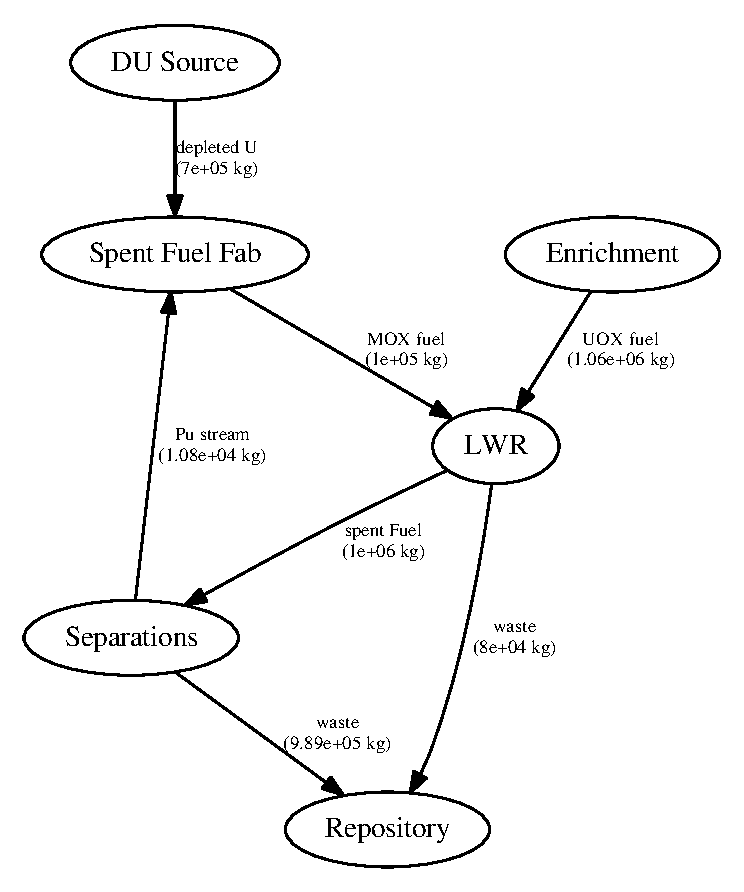
\includegraphics{./images/flow-mod-open-1.eps}
\end{center}
\end{figure}

To switch to a fully closed fuel cycle, all that needs to be done is change
the output commodity for the \Class{BatchReactor}'s spent MOX fuel.  All this
requires is a one-word change in the input file: 

\begin{lstlisting}[language=diff]
  --- mod-open-1.xml	2014-10-08 08:31:33.892523173 -0500
  +++ closed-1.xml	2014-10-08 08:31:33.892523173 -0500
  @@ -108,7 +108,7 @@
           <fuel>         
             <incommodity>mox_fuel</incommodity>
             <inrecipe>lwr_mox_fuel</inrecipe>
  -          <outcommodity>spent_mox</outcommodity>
  +          <outcommodity>spent_fuel</outcommodity>
             <outrecipe>mox_spent_fuel</outrecipe>
           </fuel>
\end{lstlisting}

This results in new the material flows in Figure \ref{fig:flowclosed}. Note
that because the \Class{BatchReactor} always transmutes fuel into the same
composition, the nuclide level flows are not very realistic for the full, multipass
recycle case.

\begin{figure}[H]
\label{fig:flowclosed}
\caption{Full MOX recycle (multi-pass) fuel cycle material flows.}
\begin{center}
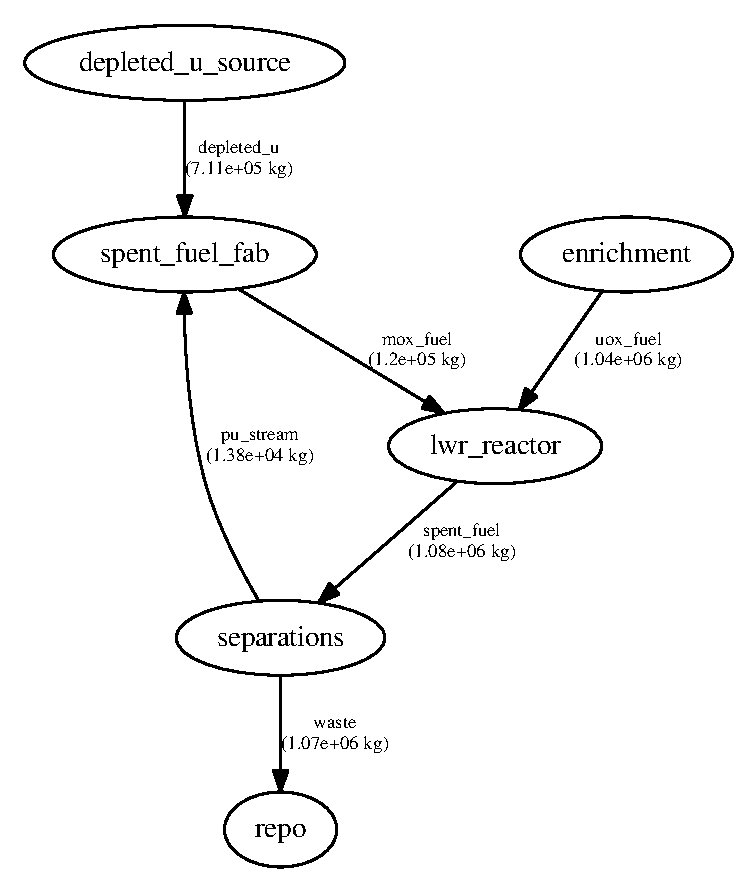
\includegraphics{./images/flow-closed-1.eps}
\end{center}
\end{figure}

Figure \ref{fig:puseries1} shows the full-system plutonium buildup for open
(no recycle), modified open, and closed (infinite-pass recycle) variations of
the scenario described above (all just a single reactor).  The figure was
generated directly from \Cyclus output data. After several batch cycles (near
month 300) in the modified open and closed cases, enough separated fissile
material accumulates in the fuel fabrication facility to generate a full
recycled batch.  When this batch is transmuted, more plutonium is burned than
created.  This results in a drop in the total fuel cycle system plutonium
inventory.  This pattern repeats roughly every 10 cycles (200 months) for the
modified open case and every 9 cycles (180 months) for the closed case.
Because the modified open scenario does not re-recycle material, it takes the
fabrication facility 1 cycle longer to accumulate a full batch worth of
fissile material.  Because facilities are represented individually and
transact discrete materials as discrete events, realistic non-uniform patterns
in facility behavior can be observed affecting total system behavior in ways
that are less commonly observed in fleet-based, continuous material flow
modeling.

\begin{figure}[H]
\label{fig:puseries1}
\caption{System plutonium buildup with one reactor.}
\begin{center}
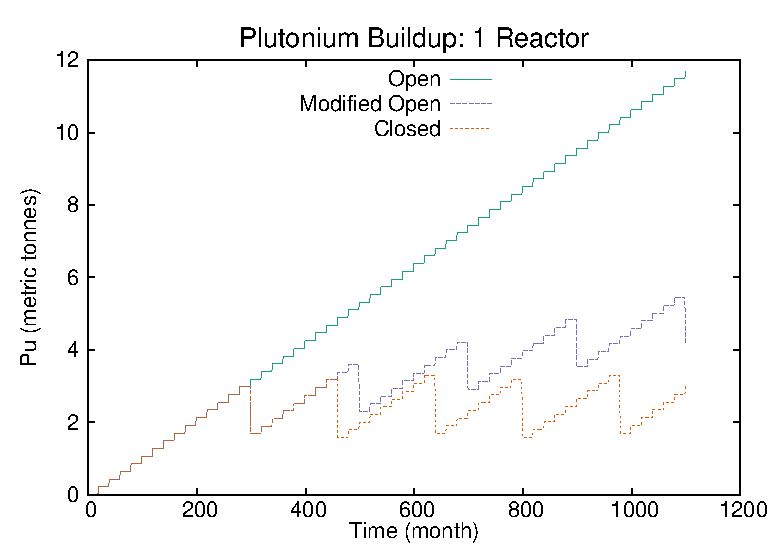
\includegraphics{./images/puseries-1.eps}
\end{center}
\end{figure}

The open, modified open, and closed scenarios can easily be modified to have
several reactors each with staggered refueling times.  As the number of
reactors increases, the behavior of the system approaches a more steady
average reminiscent of continuous material flow models.  The plutonium buildup
for these three multi-reactor variations is shown in Figure
\ref{fig:puseriesn}.

\begin{figure}[H]
\label{fig:puseriesn}
\caption{System plutonium buildup with staggered refueling for many reactors.}
\begin{center}
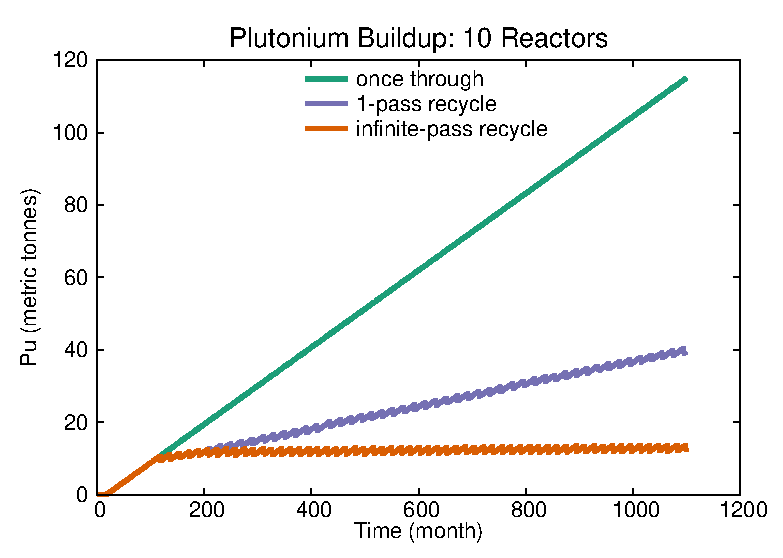
\includegraphics{./images/puseries-n.eps}
\end{center}
\end{figure}

